\subsection{Terrain Generation}

\begin{table}[H]
 \centering
 \begin{tabular}{lllll}
  \textbf{Input} & & \textbf{Function} & & \textbf{Output} \\
  \midrule
  \textit{Size, Offset, SeaLevel} & $\rightarrow$ & \textbf{TerrainGenerator} & $\rightarrow$ & \textit{Terrain} \\
  \bottomrule
 \end{tabular}

 \caption{Definition of the TerrainGenerator function which is responsible for generating the terrain.}
 \label{table:terrgen}
 \end{table}
\vspace{-0.4cm} % Mimic spacing below figures


The terrain generator constructs the landscape on which the city can be assembled.
It generates a mesh congregated out of triangles and a Perlin noise generator to apply height to the triangles' connection points.
Naturally, other generators need to take into account the height of the terrain and avoid uninhabitable areas like water and very steep hills.
The mesh is then textured by applying one texture to the terrain.
Colours of the texture blends between other colors depending on the height level of the terrain and water to illustrate the ground type at the current height level.

Cities could have been generated on a flat plane, which does have its advantages since more time could be spent on additional aesthetic details for the city.
However, a city surrounded by a landscape would result in a more realistic and vivid setting, which would indirectly make the city look better than if it were generated on a flat surface.
A plane that could simulate a basic, yet somewhat realistic, environment for the city to be generated upon was a self-evident feature that would be included in the project.
The generated environment would be decided to be referred to as terrain.
This terrain would be based on real-world aesthetics and therefore include natural biomes such as snowy mountains, grassland, hills and bodies of water, specifically oceans/lakes.
Additional aspects would bypass the range of the project's goals since the core focus of this project was the city, not the terrain.
Therefore, a decision was made to keep the terrain looking rather primitive, i.e. that it would be limited and expected to include: 

\begin{easylist}
 @ A mesh to represent the ground.
 @ The terrain's shape, as in bumps, hills, and valleys.
 @ A simple, flat plane clipping through the terrain to represent water.
 @ Colour and texture for water and ground depending on the height of a certain point on the terrain.
\end{easylist}

There were two ways the terrain base could have been created: either using a custom mesh made of triangles, or using an advanced, built-in terrain mesh API provided by Unity.
Both options had their advantages and disadvantages.

\begin{figure}[H]
  \centering
  % Use two minipages to add padding for the figure and its caption
  \begin{minipage}{.45\textwidth}
    \centering
    \begin{minipage}{.9\textwidth}
      \centering
      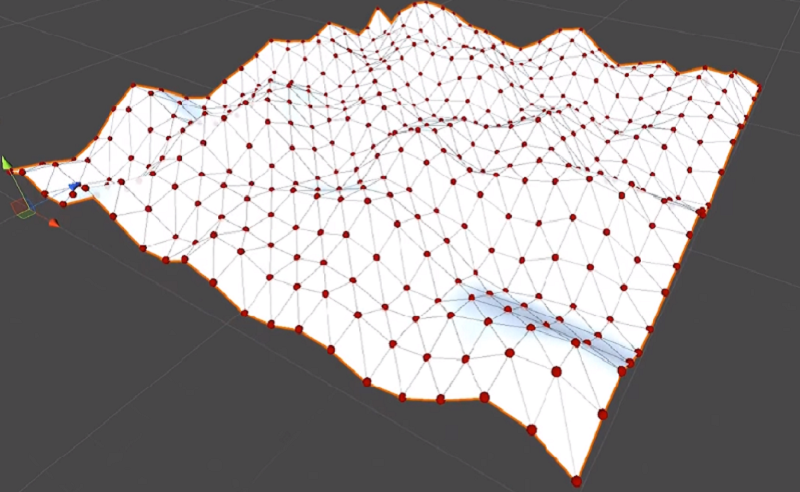
\includegraphics[width=\textwidth]{figure/terrain_mesh.png}
      \caption{Visualization of the mesh. The triangles in this picture are scaled up greatly.}
      \label{fig:terrmesh}
    \end{minipage}
  \end{minipage}
  \begin{minipage}{.45\textwidth}
    \begin{minipage}{.9\textwidth}
      \centering
      \centering
      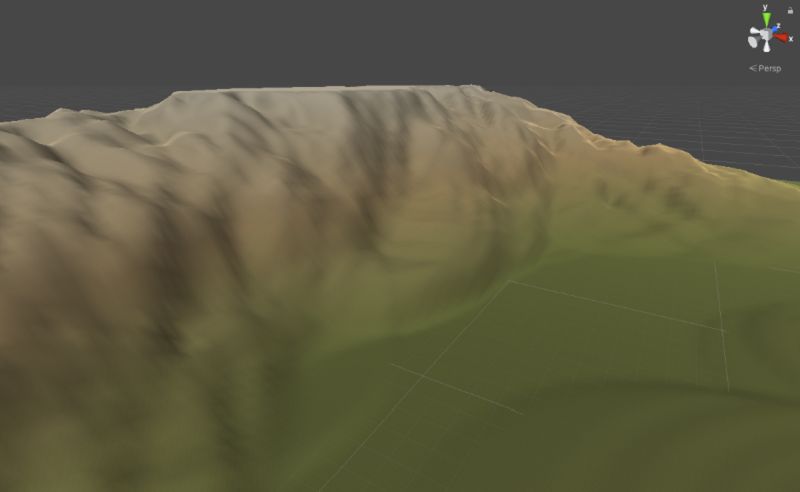
\includegraphics[width=\textwidth]{figure/terrain_API.png}
      \caption{Preview of a primitive terrain mesh using Unity Terrain API.}
      \label{fig:terrAPI}
    \end{minipage}
  \end{minipage}
\end{figure}

Meshes consists of triangles connected to one another, similar to \ref{fig:terrmesh}.
However, height-based texture splatting could be problematic using this alternative, for the reason that a custom shader would have to be coded that performs the blending of textures.
This would lead to issues when exporting the terrain, along with the fact that more programming has to be done for this task.
On the other hand, the API is easy to get started with, because of its extensive documentation to encompass its functionalities.
For instance, texture splatting is incorporated into the API, which would make the process of generating textures much simpler.

In the first iteration for the terrain base, the API by Unity seemed reasonable as a primary choice due to its simplicity and availability.
Unfortunately, the API did not produce traditional meshes, and instead produced dynamically adapting objects specific to Unity.
Converting the object could be done using Unity Editor packages; however, those tools would be inaccessible when compiling the final application, and including them in it did not seem possible.
Because of this, the terrain was refabricated with a custom mesh.
To counteract the need to program a custom shader, the terrain only contained one texture, which was gradually saturated with a different color to illustrate the expected type of ground existing on that height level.
Specifically, the texture's color would be shifted toward a white color to illustrate mountain tops, brown color for hills, green for low ground grassland, and a beige-yellow color for heights slightly above water.
Water is unaffected by this.

The next decision was to pick an algorithm that could designate height levels for the flat terrain, i.e. to shape it with inward and outward-facing dents that would represent valleys/ocean and mountains, respectively.
It was decided that the terrain was to be procedurally generated, as it would allow drastically more varied content in the generator.
The most common algorithms considered that could solve the procedurally generated landscape were simplex noise and Perlin noise.
If the height value from one of these functions were applied to the height value of each point, it would shape the terrain in a way similar to the real world.

Finally; appearance.
A blank, white canvas would not be appropriate as an environment, as it would appear glaringly unrealistic.
Therefore textures were implemented to grant the terrain the appearances of grass, mountains, water, etc. to showcase their existence, coloured as explained previously.
These following bullet points were the goals for the appearance of the terrain:

\begin{easylist}
 @ Oceans and lakes should have a blue tint.
 @ Terrain slanting towards oceans with low steepness should transition into beaches.
 @ Spacious plains should cover various shades of green.
 @ Mountains should appear rocky.
 @ Tall mountain peaks should be covered in snow.
\end{easylist}

